\section{Conclusión y trabajos a futuro}

\begin{subsection}{Conclusión}

	\begin{frame}\frametitle{Conclusión}
		\begin{itemize}\addtolength{\itemsep}{5mm}
			\item La nueva capa de distribución, junto con el rediseño efectuado, mantiene compatibilidad con el modelo original de \fud.
			\pause
			\item Los desarrolladores pueden implementar aplicaciones clientes de FuD-BOINC que pueden correr tanto en 
			Linux como en Windows.
			\pause
			\item FuD-BOINC debería ser utilizado por aplicaciones que requieran gran cantidad de procesamiento.
			\pause
			\item La investigación realizada permitió desenvolvernos satisfactoriamente ante un tema desconocido: computación 
			voluntaria con BOINC.
		\end{itemize}
	\end{frame}

\end{subsection}


\begin{subsection}{Trabajos a futuro}

	\begin{frame}\frametitle{Trabajos a futuro}
		\begin{itemize}\addtolength{\itemsep}{5mm}
			\item Instruir y profundizar los conocimientos sobre la administración y configuración de un proyecto BOINC.
			\item Lanzar oficialmente un proyecto de computación voluntaria \textbf{FuDePAN@HOME}.
			\item Implementar un screensaver con un logo personalizado de FuDePAN.
			\item Agregar la entrega de créditos a los clientes respecto de la cantidad de trabajos procesados.			
		\end{itemize}
	\end{frame}
		
	\begin{frame}\frametitle{Trabajos a futuro}
		\begin{itemize}
			\item Integrar el funcionamiento de las nuevas capas \textbf{L3} y \textbf{L4} de \fud \ con esta capa de distribución.
		\end{itemize}	
		\begin{center}
			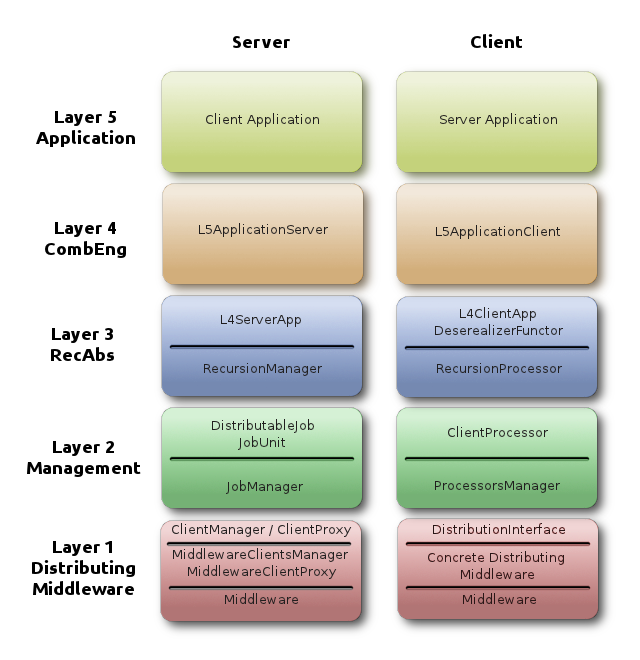
\includegraphics[scale=0.26]{images/fud-l4.png}
		\end{center}
	\end{frame}
	
	\begin{frame}
		\centerline{\Huge{\textbf{¿Preguntas?}}}
	\end{frame}
	
	\begin{frame}
		\centerline{\Huge{\textbf{¡Gracias!}}}
	\end{frame}

\end{subsection}

